
\documentclass[11pt,letterpaper]{article}
\usepackage[margin=0.86in,top=0.8in,bottom=0.86in,headheight=15pt]{geometry}
\usepackage{fontspec}
\setmainfont{texgyrepagella}[Extension=.otf,UprightFont=*-regular,ItalicFont=*-italic,BoldFont=*-bold,BoldItalicFont=*-bolditalic]
\setmonofont{lmmono10-regular.otf}[Scale=0.86]
\usepackage{amsmath,amssymb}
\usepackage{unicode-math}
\setmathfont{texgyrepagella-math.otf}
\AtBeginDocument{\let\setminus\smallsetminus}
\usepackage{microtype}
\usepackage{graphicx}
\usepackage{float}
\usepackage[font=small,labelfont=bf]{caption}
\usepackage{placeins}
\usepackage{needspace}
\usepackage{longtable,booktabs,array,calc}
\usepackage{xcolor}
\definecolor{Accent}{HTML}{1B4965}
\definecolor{Muted}{HTML}{58656D}
\usepackage{xurl}
\usepackage{hyperref}
\usepackage{bookmark}
\hypersetup{colorlinks=true,urlcolor=Accent,linkcolor=Accent,citecolor=Accent,
pdftitle={A verified spectral bound for Pauli contextuality: independent validation and critical synthesis},
pdfauthor={Hoggar Bound Lab; AI-assisted research artifact},
pdfsubject={Independent verification companion; research preprint, not peer reviewed}}
\urlstyle{same}
\usepackage{fancyhdr}
\pagestyle{fancy}
\fancyhf{}
\fancyhead[L]{\small\color{Muted}HOGGAR BOUND LAB}
\fancyhead[R]{\small\color{Muted}Independent validation}
\fancyfoot[L]{\footnotesize\color{Muted}Research preprint \textbullet\ 2026-11-09}
\fancyfoot[R]{\footnotesize\color{Muted}\thepage}
\renewcommand{\headrulewidth}{0.25pt}
\renewcommand{\footrulewidth}{0pt}
\usepackage{titlesec}
\titleformat{\section}{\large\bfseries\color{Accent}}{}{0pt}{}
\titlespacing*{\section}{0pt}{1.05em}{0.4em}
\setcounter{secnumdepth}{-2}
\setlength{\parindent}{0pt}
\setlength{\parskip}{0.45em}
\setlength{\emergencystretch}{3em}
\widowpenalty=10000
\clubpenalty=10000
\brokenpenalty=10000
\setlength{\LTleft}{0pt}
\setlength{\LTright}{0pt}
\setlength{\tabcolsep}{4pt}
\renewcommand{\arraystretch}{1.14}
\providecommand{\tightlist}{\setlength{\itemsep}{0pt}\setlength{\parskip}{0pt}}
\begin{document}
\thispagestyle{empty}
{\small\bfseries\color{Accent}INDEPENDENT VERIFICATION COMPANION}\par
\vspace{0.6em}
{\fontsize{22}{25}\selectfont\bfseries A verified spectral bound\\for Pauli contextuality}\par
\vspace{0.25em}
{\large\color{Accent}Independent validation and critical synthesis}\par
\vspace{0.8em}
{\normalsize Hoggar Bound Lab; AI-assisted research artifact}\par
{\small\color{Muted}2026-11-09 \quad\textbullet\quad Research preprint, not peer reviewed}\par
\vspace{0.6em}
{\color{Accent}\hrule height 0.65pt}
\vspace{0.5em}
\section{Abstract}\label{abstract}

We independently validate and formalize a spectral lower bound for Pauli contextuality. Jonah's October 2026 preprints already give the cubic-trace method and the identical spectral bound for the full symplectic and quadric families {[}12,13{]}. The present statement allows arbitrary subsets of nonidentity tensor-Pauli observables with all their induced commuting contexts. The signed context score equals the third trace moment of a Hermitian Pauli sum; the classical sharp cubic-moment inequality then yields a violated fraction of at least \(1/2-\sqrt{D+1}/(D+2)\) for the full configuration in dimension \(D=2^N\). The general theorem and finite corollaries have been checked in Lean 4, including an exact three-qubit minimum of 63 with a kernel-evaluated witness. Independent matrix validation compares 138,792 contexts, recounts eight witnesses, and checks 120 sparse supports. Focused Moonlab, QGTL, quantum\_rng and Eshkol experiments connect this mathematics to executable examples. The five-qubit hyperbolic result established here is \(d\ge6426>4743\), not an exact-degree proof; prior work claims the stronger value 6975. We claim a reproducible verification artifact, with explicit formal and computational boundaries, rather than priority for the spectral bound.

\section{1. Problem and mathematical model}\label{problem-and-mathematical-model}

Quantum contextuality obstructs a single assignment of outcomes that respects every compatible measurement relation. For Pauli observables, this becomes a finite signed constraint problem. De Boutray and collaborators formalized its contextuality degree as the minimum number of violated constraints {[}1{]}. This note concerns one precise family: all commuting lines induced by a selected set of nonidentity tensor-Pauli operators.

Let \(N\ge1\), \(D=2^N\), and \(V=\mathbb F_2^N\times\mathbb F_2^N\). A label \(v=(x,z)\) represents the Hermitian operator

\[P_v=i^{\sum_jx_jz_j}X^xZ^z,\]

equivalently a tensor product of \(I,X,Z,Y\), with \(Y=iXZ\). The symplectic form

\[[u,v]=x_u\cdot z_v+z_u\cdot x_v\]

determines commutation. A context is an unordered triple \(\ell=\{u,v,u+v\}\) of distinct nonzero labels with \([u,v]=0\). Its sign \(s_\ell\in\{\pm1\}\) is defined by \(P_uP_vP_{u+v}=s_\ell I\).

Choose \(S\subseteq V\setminus\{0\}\) and include every such context contained in S. Write \(m=|S|\), \(L=|\mathcal L(S)|\). A deterministic noncontextual assignment \(f:S\to\{\pm1\}\) violates a context when its three assigned values multiply to \(-s_\ell\). If \(v(f)\) counts violations, its signed score is

\[\beta(f)=\sum_{\ell\in\mathcal L(S)}s_\ell\prod_{u\in\ell}f(u)
=L-2v(f),\qquad d(S)=\min_fv(f).\]

The induced-context requirement is essential. The argument below does not automatically apply to an arbitrary subset of contexts on the same points. It also concerns these observable-product constraints, rather than every formalization of operational contextuality.

\section{2. Trace moments and the spectral bound}\label{trace-moments-and-the-spectral-bound}

Define \(A_f=\sum_{u\in S}f(u)P_u\). Pauli orthogonality and omission of the identity imply

\[\operatorname{tr}A_f=0,\qquad \operatorname{tr}A_f^2=Dm.\]

Expanding the cube gives the key identity

\[\boxed{\operatorname{tr}A_f^3=6D\beta(f).}
\tag{1}\]

Terms whose three labels do not sum to zero have zero trace. A zero-sum triple of distinct commuting labels contributes the same signed value in all six orders. For anticommuting labels, opposite orders cancel. These exhaust the possibilities because S excludes zero. Thus the factor six records the six ordered representatives of an unordered line. The trace identity appears in Jonah {[}12, Theorem 1; 13, Section 7{]}. The cancellation argument here makes explicit that line-closure of S is unnecessary for this trace statement.

For completeness, the analytic step admits a short elementary proof. Let \(\lambda_1,\ldots,\lambda_n\in\mathbb R\) satisfy \(\sum_i\lambda_i=0\), \(\sum_i\lambda_i^2=nm\), with \(n\ge2\). Put \(a=\sqrt{(n-1)m}\). Cauchy--Schwarz applied to the other \(n-1\) entries gives

\[\lambda_i^2\le(n-1)(nm-\lambda_i^2),\]

so \(|\lambda_i|\le a\). Consequently,

\[0\le\sum_i(a-\lambda_i)
\left(\lambda_i+\frac{a}{n-1}\right)^2
=\frac{nm(n-2)a}{n-1}-\sum_i\lambda_i^3.
\tag{2}\]

This is the classical sharp cubic-moment, or Okumura, inequality {[}6,7{]}. Jonah {[}12, Lemma 5 and Theorem 6{]} applies the same extremal spectrum to contextuality. Applying it to the D real eigenvalues of \(A_f\), then using (1), yields

\[\boxed{\beta(f)\le B(D,m)
=\frac{(D-2)m^{3/2}}{6\sqrt{D-1}}.}
\tag{3}\]

Therefore

\[\boxed{d(S)\ge\left\lceil\frac{L-B(D,m)}2\right\rceil.}
\tag{4}\]

\Needspace{7\baselineskip}
The zero-support case is trivial. For nonempty S, equality in the nondegenerate spectral bound requires one positive eigenvalue \(a\) and D−1 equal negative eigenvalues \(-a/(D-1)\). Thus \(A_f=c(D|\psi\rangle\langle\psi|-I)\), with \(c=\sqrt{m/(D-1)}\). Pauli orthogonality then gives expectations \(\langle P_u\rangle=f(u)/c\) on S and zero outside S. This explains why flat Pauli expectation vectors produce saturation examples. The equality characterization is mathematical exposition here; it is not among the audited Lean equality theorems.

\section{3. Finite consequences and exact rounding}\label{finite-consequences-and-exact-rounding}

For the full space \(W(2N-1,2)\), \(m=D^2-1\) and \(L=(D^2-1)(D^2-4)/12\). For \(N\ge2\), equation (4) implies

\[\frac{d(W)}L\ge\frac12-\frac{\sqrt{D+1}}{D+2}.
\tag{5}\]

For the real Pauli set, consisting of words with an even number of Y factors, the induced geometry is \(Q^+(2N-1,2)\). Its counts are

\[m=\frac{(D-1)(D+2)}2,\qquad
L=\frac{(D-1)(D+2)(D-2)(D+4)}{48}.\]

Substitution into (4) gives the same fractional expression as (5) with D replaced by D/2. These are lower bounds; except when a matching witness is available, they leave an optimization gap.

{\def\LTcaptype{table} % do not increment counter
\begin{longtable}[]{@{}
  >{\raggedright\arraybackslash}p{(\linewidth - 8\tabcolsep) * \real{0.3200}}
  >{\raggedleft\arraybackslash}p{(\linewidth - 8\tabcolsep) * \real{0.1700}}
  >{\raggedleft\arraybackslash}p{(\linewidth - 8\tabcolsep) * \real{0.1700}}
  >{\raggedleft\arraybackslash}p{(\linewidth - 8\tabcolsep) * \real{0.1700}}
  >{\raggedleft\arraybackslash}p{(\linewidth - 8\tabcolsep) * \real{0.1700}}@{}}
\toprule\noalign{}
\begin{minipage}[b]{\linewidth}\raggedright
Configuration
\end{minipage} & \begin{minipage}[b]{\linewidth}\raggedleft
Points
\end{minipage} & \begin{minipage}[b]{\linewidth}\raggedleft
Contexts
\end{minipage} & \begin{minipage}[b]{\linewidth}\raggedleft
Checked lower bound
\end{minipage} & \begin{minipage}[b]{\linewidth}\raggedleft
Recounted witness
\end{minipage} \\
\midrule\noalign{}
\endhead
\bottomrule\noalign{}
\endlastfoot
\(W(5,2)\), three qubits & 63 & 315 & 63 & 63 \\
\(W(7,2)\), four qubits & 255 & 5,355 & 1,451 & 1,575 \\
\(W(9,2)\), five qubits & 1,023 & 86,955 & 28,786 & 31,479 \\
\(Q^+(7,2)\), four qubits & 135 & 1,575 & 315 & 315 \\
\(Q^+(9,2)\), five qubits & 527 & 23,715 & 6,426 & 6,975 \\
\end{longtable}
}

All lower bounds in this table have audited Lean corollaries. Witness entries are direct computational recounts in the independent validator. The three-qubit full-space witness and its exact minimum are additionally kernel checked. A witness proves an upper bound on the minimum; finding it repeatedly does not establish optimality. Matching lower and upper bounds establish the four-qubit hyperbolic value within the combined mathematical/computational evidence.

The numerical checker avoids floating-point ceilings. Since \(B^2=(D-2)^2m^3/[36(D-1)]\), it uses an integer square root of the quotient to bound the integer score β, then adjusts to the required parity \(\beta\equiv L\pmod2\). In particular,

\[d(Q^+(9,2))\ge6426>4743=23715/5.
\tag{6}\]

This excludes an L/5 value in that instance. It does \textbf{not} prove \(d=6975\). The provenance of the stronger external claim is discussed below.

The general formula also supplies an asymptotic mathematical consequence. Uniformly random independent signs violate each context with probability one half, so some assignment has at most L/2 violations. Combining this upper bound with (5) squeezes the full-space fraction to \(d(W)/L\to1/2\). This is an analytic deduction, not a fit to the finite table; the limit itself was not included in the audited Lean scope.

\begin{figure}[H]
\centering
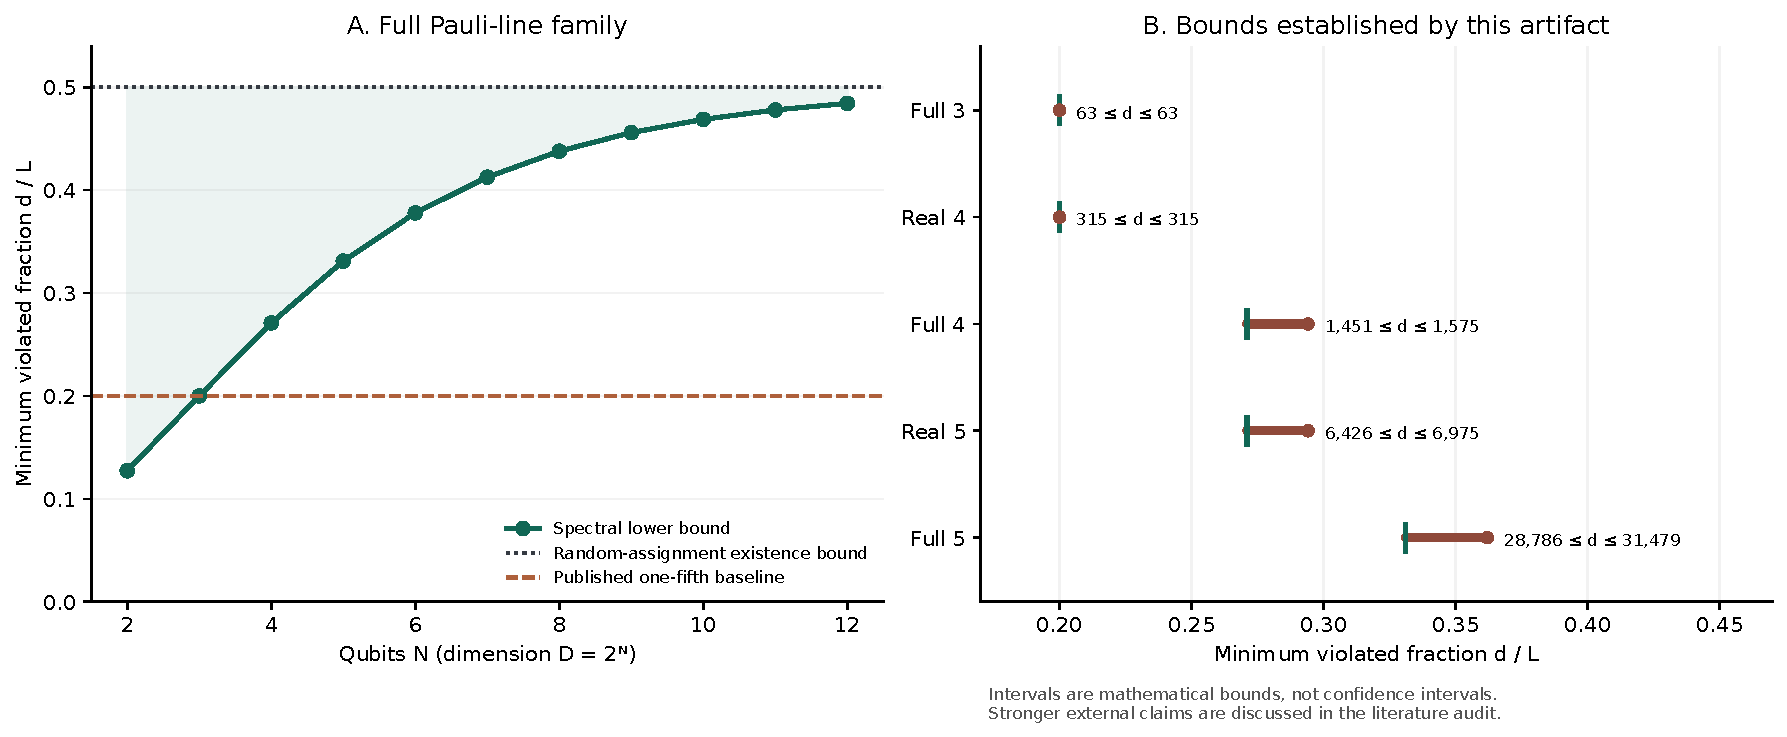
\includegraphics[width=1\linewidth,height=\textheight,keepaspectratio,alt={Spectral bounds and finite verification. Left: the analytic full-space lower curve, the published one-fifth baseline, and the random-assignment existence upper bound. Right: intervals established by this artifact. These are mathematical bounds, not confidence intervals or a statement of the strongest external claims.}]{independent-figures/spectral-bounds.pdf}
\caption{Spectral bounds and finite verification. Left: the analytic full-space lower curve, the published one-fifth baseline, and the random-assignment existence upper bound. Right: intervals established by this artifact. These are mathematical bounds, not confidence intervals or a statement of the strongest external claims.}
\end{figure}

\FloatBarrier
\section{4. Formal verification boundary}\label{formal-verification-boundary}

The audited development uses Lean 4.35.0 and Mathlib 4.35.0. Six original modules were freshly rechecked from source, and \texttt{lake\ build} succeeded. The development constructs Pauli matrices, proves their products and traces, establishes (1), transfers the real spectral inequality to matrices, counts configurations, and derives finite bounds. The main theorem is \texttt{HoggarBound.hoggar\_bound}; representative consequences include \texttt{full\_space\_fraction}, \texttt{four\_qubit\_contexts}, and \texttt{five\_qubit\_hyperbolic\_contexts}.

The printed axiom dependencies for all 22 audited declarations were exactly \texttt{propext}, \texttt{Classical.choice}, and \texttt{Quot.sound}. The supplementary module \path{HoggarBound/IndependentWitness.lean} checks an explicit three-qubit assignment with 378 violated ordered flags, using \texttt{decide\ +kernel} rather than native evaluation. \texttt{IndependentContexts.lean} proves that each violated unordered context contributes exactly six flags. The entry point \texttt{IndependentVerification.lean} combines this certificate with the analytic lower bound: \texttt{three\_qubit\_exact\_minimum} proves both existence of an assignment with exactly 63 violations and the universal lower bound 63. \texttt{three\_qubit\_total\_contexts} proves that the model has 315 contexts.

Supplementary checked statements also exclude assignments below 6426 and the five-qubit hyperbolic L/5 value. The source-build and axiom evidence is in \path{results/lean-source-recheck.log} and \path{results/lean-independent-verification.log}.

This verifies the stated mathematics in the formal model, including the historical exact three-qubit result. It does not certify that every explanatory sentence is formalized, that numerical software has no defects, or that the result is historically new. The guaranteed scope excludes a general equality classification, the Kramers extension, asymptotic convergence, and exact optima beyond the explicitly certified case.

\section{5. Independent validation and falsification controls}\label{independent-validation-and-falsification-controls}

\path{tests/independent_validation.py} obtains the one-qubit multiplication table from literal 2×2 matrices and constructs tensor products directly. It does not copy the C engine's bit-phase multiplication formula. Across the full, hyperbolic and elliptic families for N=2,\ldots,5, every generated context and sign agrees with the C output: \textbf{138,792 contexts across twelve configurations}. Eight witness files are decoded and recounted, with content hashes recorded in \path{results/independent_validation.json}.

The unnormalized Hoggar vector is

\[h=(-1+2i,1,1,1,1,1,1,1)^T,
\qquad h^\dagger h=12.\]

Every nonidentity expectation numerator \(h^\dagger P_uh\) has absolute value four. Thus normalized expectations have modulus 1/3. Their sign assignment violates 63 contexts, and its operator satisfies \(\operatorname{tr}A^2=504\), \(\operatorname{tr}A^3=9072\), with numerical spectrum \(\{21,-3^{\times7}\}\). The integer-valued operations are exactly representable at these sizes; the spectral decomposition is a floating-point cross-check. The violated-line incidence graph is connected, cubic, and has 126 vertices, 189 edges, diameter six, and girth twelve, consistent with the split Cayley hexagon structure previously identified in the literature {[}2{]}.

Realifying h by concatenating its real and imaginary coordinates produces a four-qubit state with modulus 1/3 on all 135 real nonidentity Paulis and zero on the other nonidentity Paulis. Its sign assignment violates 315 of the 1575 real contexts.

The validator additionally tests 120 randomly selected sparse supports at three and four qubits. The observed cubic-trace residual is exactly zero in all trials. A deliberate context-sign mutation changes the score and breaks the trace identity, providing a positive control that detects a specified inconsistency. These checks improve confidence in the implementation; finite tests cannot replace the universally quantified Lean theorem. The checker explicitly rejects optimized Python execution, which would disable its assertions.

\section{6. Operational experiments with the Tsotchke stack}\label{operational-experiments-with-the-tsotchke-stack}

The stack evidence is recorded separately in \path{results/stack_audit.json}, with compiler/runtime versions and binary or output hashes. Each component has a specific, limited role.

\textbf{Moonlab} provides classical state-vector simulation. The audit checks separately generated runner output covering 17,055 ideal context trials. This exercises a simulated measurement path connected to the contextuality construction. It supplies neither physical quantum measurements nor evidence of hardware quantum advantage. Statistical significance labels in noisy simulations were outside this audit.

\textbf{QGTL} contributes the Fubini--Study metric and Berry-curvature derivative kernels. For the normalized Hoggar state and 63 Pauli-generated parameters, the metric diagonal is 2/9 and its numerical rank is 14, consistent with the real tangent dimension of complex projective space \(\mathbb{CP}^7\). Its fourteen nonzero eigenvalues are approximately one. Maximum disagreements against independent reference formulas were \(1.39\times10^{-17}\) for the metric and \(5.55\times10^{-17}\) for curvature. Twenty random cases and a phase-gauge check also passed, with errors below \(7.2\times10^{-15}\).

There is a concrete bridge to the constraint structure. For derivatives \(\partial_u\psi=-iP_u\psi/2\), the quantum geometric tensor is \(Q_{uv}=(\langle P_uP_v\rangle-\langle P_u\rangle\langle P_v\rangle)/4\). At the Hoggar state, commuting satisfied and violated pairs have metric magnitudes 1/18 and 1/9 respectively. The implementation reported no context-classification mismatches. Only these normalized pure-state kernels were audited; distributed execution, GPU behavior, and the rest of QGTL were not qualified.

\textbf{quantum\_rng} is a classical quantum-inspired software mixer. A 4096-byte stream repeated under the same build and seed 20261109, while a different seed changed the stream. This establishes the tested reproducibility behavior, not physical entropy, cryptographic security, statistical certification, or cross-platform bitwise identity.

\textbf{Eshkol} v1.3.6-evolve independently evaluates integer rounding certificates for the five principal finite bounds and a Hoggar spectral moment identity. Those checks passed. This provides a separate executable arithmetic path; it is not a substitute for the Lean kernel proof.

\section{7. Prior work, contribution and limitations}\label{prior-work-contribution-and-limitations}

The values 63 for the full three-qubit configuration and 315 for the four-qubit hyperbolic quadric are established results {[}2,4{]}. Muller and collaborators provide the principal published heuristic witnesses used for comparison {[}3{]}. Li, Gupta and Ganesh's October 2026 paper includes a Lean proof of the latter value and asks about the five-qubit value 4743 {[}4{]}. Those achievements must not be attributed to this artifact.

Jonah's 21 October 2026 preprint {[}12, Theorem 6{]} already states exactly equation (3) for the full and quadric families, together with an elliptic refinement and equality conditions. Its Theorem 8 determines when those spectral floors are attained. The preceding preprint {[}13, Section 7{]} also uses the cubic-trace identity and spectral relaxation. These primary PDFs were read directly. The spectral method and family bounds are therefore prior work. Their stated scope does not give the arbitrary, potentially non-line-closed S formulation used here; dropping that hypothesis for the trace identity is a modest generalization, for which no priority claim is made.

Jonah's earlier deposit {[}5{]} claims computer-assisted exact degrees 315, 1575 and 6975 for the four-qubit elliptic, four-qubit full, and five-qubit hyperbolic configurations. We replayed its supplied exact certificate verifier successfully, but did not rerun its exhaustive census. A separate digest {[}14{]} announces stronger five-qubit full and elliptic lower bounds of 28830 and 6510, with proofs and code held privately. We do not independently certify those announcements. These deposits are not peer reviewed; their existence nevertheless rules out describing this artifact's bounds as the first or strongest results.

Hoggar SIC geometry and cubic purity relations also have substantial prior literature {[}8{]}. Tensor-Pauli-covariant maximal equiangular constructions are restricted to one and three qubits {[}9{]}; this restriction does not prohibit other SIC covariance groups. More general contextuality constructions and stabilizer-testing games already exhibit strong separations {[}10,11{]}. Our full-Pauli asymptotic statement does not resolve the specific repeated-graph-family limit question posed in {[}10{]}.

The elliptic refinement using Kramers degeneracy is already explicit in {[}12{]} and remains outside this artifact's audited formal proof. It requires an antiunitary \(\theta\) with \(\theta^2=-I\) and \(\theta A_f\theta^{-1}=A_f\); setwise invariance of S alone is insufficient. Reducing paired eigenvalues to dimension D/2 yields the computationally reported elliptic lower bounds 9, 291 and 6501 for N=3,4,5. Its equality object is a normalized rank-two projector, rather than a pure state supported only on the elliptic observables.

The supported contribution is a Lean formalization of the spectral bound with an explicit arbitrary-support scope, checked finite corollaries, a kernel-checked three-qubit witness, independent executable validation, and a delimited stack demonstration. Bounded literature searches do not establish priority even for the formalization. This companion is a theoretical analysis and critical synthesis, not a statistical meta-analysis of pooled experiments. Physical validation, broader software qualification, further exact optima, and independent scholarly review remain distinct tasks.

\clearpage
\section{References and evidence}\label{references-and-evidence}

\begin{enumerate}
\def\labelenumi{\arabic{enumi}.}
\tightlist
\item
  H. de Boutray, F. Holweck, A. Giorgetti, P.-A. Masson and M. Saniga. \emph{Contextuality degree of quadrics in multi-qubit symplectic polar spaces}. J. Phys. A 55 (2022), 475301. \href{https://arxiv.org/abs/2105.13798}{Corrected arXiv record}; \href{https://doi.org/10.1088/1751-8121/aca36f}{DOI}.
\item
  A. Muller, M. Saniga, A. Giorgetti, H. de Boutray and F. Holweck. \emph{New and improved bounds on the contextuality degree of multi-qubit configurations}. MSCS 34 (2024), 322--343. \href{https://arxiv.org/html/2305.10225v3}{Full text}; \href{https://doi.org/10.1017/S0960129524000057}{DOI}.
\item
  A. Muller, M. Saniga, A. Giorgetti, F. Holweck and C. Kelleher. \emph{A new heuristic approach for contextuality degree estimates and its four- to six-qubit portrayals}. J. Phys. A 58 (2025), 215302. \href{https://arxiv.org/html/2407.02928v1}{Full text}; \href{https://doi.org/10.1088/1751-8121/add22b}{DOI}.
\item
  Z. Li, A. Gupta and V. Ganesh. \emph{The Four-Qubit Hyperbolic Quadric Has Contextuality Degree 315}. arXiv:2610.26465v1, 19 October 2026. \href{https://arxiv.org/html/2610.26465v1}{Full text}.
\item
  B. W. Jonah. \emph{A section--square law for Pauli quadrics, and an independently regenerated proof that the four-qubit elliptic quadric has contextuality degree 315}. Preprint v0.7, 20 October 2026. \href{https://zenodo.org/records/23510634}{Primary deposit}; \href{https://doi.org/10.5281/zenodo.23510634}{DOI}.
\item
  M. Okumura. \emph{Hypersurfaces and a Pinching Problem on the Second Fundamental Tensor}. Amer. J. Math. 96 (1974), 207--213. \href{https://doi.org/10.2307/2373587}{DOI}. Historical attribution; the inequality was checked in reference 7 rather than an accessible copy of the original.
\item
  H. Baltazar and E. Ribeiro, Jr.~\emph{Remarks on critical metrics of the scalar curvature and volume functionals on compact manifolds with boundary}. Pacific J. Math. 297 (2018), 29--45, equation (3-12). \href{https://msp.org/pjm/2018/297-1/pjm-v297-n1-p02-s.pdf}{Publisher PDF}; \href{https://doi.org/10.2140/pjm.2018.297.29}{DOI}.
\item
  B. C. Stacey. \emph{Geometric and Information-Theoretic Properties of the Hoggar Lines}. arXiv:1609.03075. \href{https://arxiv.org/html/1609.03075v1}{Full text}.
\item
  C. Godsil and A. Roy. \emph{Equiangular lines, mutually unbiased bases, and spin models}, Lemma 3.1. \href{https://arxiv.org/pdf/quant-ph/0511004}{Primary manuscript}.
\item
  A. Muller and M. Saniga. \emph{Automated search for highly contextual Kochen-Specker proofs}. arXiv:2609.19862v1, 17 September 2026. \href{https://arxiv.org/html/2609.19862v1}{Full text}.
\item
  W. Zhao, H. W. S. Liew, W. W. Ho, C. Liu and V. B. Bulchandani. \emph{Scalable tests of quantum contextuality from stabilizer-testing nonlocal games}. arXiv:2512.16654v2, revised 2 October 2026. \href{https://arxiv.org/abs/2512.16654}{Primary record}.
\item
  B. W. Jonah. \emph{Structure theorems for hyperplane completions in Pauli contextuality}. Preprint v0.3, 21 October 2026, Theorem 1, Lemma 5 and Theorems 6--8. \href{https://zenodo.org/records/23538829}{Primary deposit}; \href{https://doi.org/10.5281/zenodo.23538829}{DOI}.
\item
  B. W. Jonah. \emph{The reach of the section-square law: hyperplane completions of symplectic and quadric Pauli configurations}. Preprint v0.5, 20 October 2026, Section 7. \href{https://zenodo.org/records/23524332}{Primary deposit}; \href{https://doi.org/10.5281/zenodo.23524332}{DOI}.
\item
  B. W. Jonah. \emph{Results digest, 20 October 2026: multi-qubit contextuality degrees, Pauli-flat states and certification}. Preprint v1, 20 October 2026. Status announcement; proofs and code held privately. \href{https://zenodo.org/records/23518569}{Primary deposit}; \href{https://doi.org/10.5281/zenodo.23518569}{DOI}.
\end{enumerate}

Local reproducibility artifacts: \path{results/independent_validation.json}, \path{results/stack_audit.json}, \path{results/lean-source-recheck.log}, \path{results/lean-independent-verification.log}, and \path{results/literature-audit.md}. Evidence is scoped to the versions and hashes recorded in those artifacts. This independent companion does not replace the project's main manuscript.

\end{document}
